\documentclass[11pt]{article}

% ---------- Packages ----------
\usepackage[margin=1in]{geometry}
\usepackage{amsmath,amssymb}
\usepackage{booktabs}
\usepackage{graphicx}
\usepackage[numbers,sort&compress]{natbib}
\usepackage{xcolor}
\usepackage{pgfplots}
\pgfplotsset{compat=1.18}
\usetikzlibrary{calc}
\usepackage{hyperref}

% ---------- Hyperref setup ----------
\hypersetup{
    colorlinks=true,
    linkcolor={blue!70!black},
    citecolor={green!50!black},
    urlcolor={blue!80!black},
}

% ---------- Lightweight macros ----------
\newcommand{\code}[1]{\texttt{#1}}
\newcommand{\CodeWM}{\textsc{CodeWM}}
\newcommand{\KernelWM}{\textsc{KernelWM}}
\newcommand{\copycos}{\ensuremath{\mathrm{copy\_cos}}}
\newcommand{\lift}{\ensuremath{\mathrm{lift}}}

% ---------- Title ----------
\title{From Early-Loop Signal to Readout Repair:\\
       Deep Supervision and VICReg\\
       in Tiny JEPA Code Models}

\author{Eren Akbulut}

\date{Draft, April 2026}

% ==========================================================================
\begin{document}
\maketitle

% ---------- Abstract ----------
\begin{abstract}
Stabilized tiny JEPA code models prevent training collapse, but leave
open where transition information lives inside the model.  Geometry
probes show that the six-loop encoder compresses transition signal by
roughly $12\times$ across loops into an effective rank of $5/128$, and
direct delta prediction remains a genuine negative result:
consecutive code states are too similar to serve as a useful target.
Predictive deep supervision on intermediate loops raises lift over a
copy baseline by more than $+1.0$, but a discriminability probe
reveals the caveat: the high-lift readout collapses to $1.95/128$
effective rank with near-random KNN, so lift alone is gameable.
VICReg at the readout resolves this collapse, delivering
$\sim\!20\times$ improvement in readout discriminability on a
full-validation audit (N=$5000$), peaking at step 28K before monotonic
overfit.  At $1.3$M parameters, \CodeWM{} matches $125.9$M UnixCoder
on CommitPackFT edit retrieval at $10\times$ lower CPU latency.
Cross-seed runs show the peak is a single-seed optimum with
$2\text{--}3\times$ KNN variance: the encoder is consistently
repaired across seeds, but predictor effective rank
($5\text{--}6/128$) is the binding bottleneck.  The contribution is a
mechanism claim: intermediate-loop signal must be preserved and the
readout explicitly regularized, or prediction quality is a collapsed
space-translation artifact.
\end{abstract}

% ---------- Main body ----------
\section{Introduction}
\label{sec:introduction}

Git histories turn software into a dynamical system: a repository moves
through states as commits apply edits.  The first \CodeWM{} preprint
studied whether a tiny JEPA-style model could learn this transition
process from code states and edit actions, and found a practical
stability barrier.  Under the usual fast EMA target update, training hit
a repeatable 700-step ceiling because the target encoder collapsed; a
near-static target encoder fixed that failure and enabled stable
15K-step latent edit prediction~\citep{akbulut2026collapse}.

This paper starts after that fix.  If a tiny JEPA can be stabilized, the
next question is not merely whether it can predict the next target
embedding.  The next question is where transition information lives
inside the model, why some seemingly natural prediction objectives fail
even when training is stable, and whether the final readout remains
discriminative enough for the prediction to mean anything.

The answer is geometric.  The previous six-loop encoder does not retain
transition signal uniformly across depth.  Early loop outputs contain a
measurable edit signal, but repeated application of the shared encoder
block progressively smooths that signal away.  By the final loop,
consecutive states are almost indistinguishable under the target
encoder, deltas are tiny relative to state vectors, and the representation
space is strongly anisotropic.  In that geometry, explicitly predicting
$z_{t+1}-z_t$ is the obvious experiment and the wrong substrate.

The positive result is deep supervision.  Instead of asking the final
representation to carry every signal, we train intermediate loop outputs
to remain predictive.  The current winning configuration uses a
three-loop encoder and predictive auxiliary losses on loops 1 and 2,
while retaining the near-static EMA target and looped predictor from the
stabilized \CodeWM{} recipe.  Deep supervision repairs the loop
intermediates, but it is not sufficient by itself: a high-lift
\code{loops3-auxpred} checkpoint still collapsed the final attention-pool
readout to roughly two effective dimensions.  Adding VICReg-style
variance and covariance regularization is the current Phase~9
breakthrough because it preserves the lift while restoring a
high-rank, discriminative readout.

\paragraph{Contributions.}
\begin{enumerate}
    \item \textbf{Direct state-space delta prediction is a negative
          result, by geometry.}  Stabilized six-loop \CodeWM{}
          compresses transition signal by roughly $12\times$ across
          loops (transition-to-state norm ratio $0.123 \to 0.010$) into
          an effective rank of $5/128$.  In that geometry, early-layer
          readouts, normalized delta losses, and residual predictors
          all fail to recover a competitive predictor.  The obvious
          objective is the wrong substrate; this is a reusable
          lesson for any tiny world-model builder.
    \item \textbf{Deep supervision for looped encoders.}  Predictive
          auxiliary losses on intermediate loop outputs preserve useful
          state representations and raise lift, but also expose that
          lift alone is not a sufficient success metric.
    \item \textbf{Readout-collapse diagnostics and VICReg repair.}
          Discriminability probes show that high lift can coexist with
          online effective rank $1.95/128$ and KNN@1 near random.  On a
          full-validation audit (N=$5000$), VICReg delivers a
          $\sim\!20\times$ improvement in readout discriminability
          ($14\times$ KNN@5, $25\times$ effective rank) over the
          pre-VICReg baseline, peaking at step 28K before monotonic
          overfit.
    \item \textbf{Head-to-head against code foundation
          models~\citep{guo2022unixcoder,feng2020codebert}.}  On a paper-grade retrieval
          eval (1000 queries over a 5000-commit gallery), the
          $1.3$M-parameter step-28K \CodeWM{} matches $125.9$M
          UnixCoder: a $+0.030$ MRR edge on moderate criteria and a
          statistical tie on the strictest action-cosine threshold, at
          $10\times$ lower CPU latency.  A smaller development-scale
          benchmark dominates CodeBERT ($124.6$M) at $21\times$ lower
          latency.
    \item \textbf{Evaluation corrections and bottleneck diagnosis.}
          A 128-sample gallery inflates absolute KNN numbers
          $\sim\!12\times$ relative to a 5000-sample gallery; we
          document the inflation explicitly.  Cross-seed runs reveal
          that the peak result is a single-seed optimum
          ($2\text{--}3\times$ KNN@5 variance), and that predictor
          effective rank ($5\text{--}6/128$) is the binding bottleneck
          independent of encoder health.
\end{enumerate}

\paragraph{Status.}
This is an active draft.  Phase~8 geometry and delta-prediction results
are treated as established within the current experiment log.  Phase~9
numbers are audited on the full validation set.  The foundation-model
head-to-head uses the peak step-28K checkpoint (seed~42, pre-fix) scaled
to $1000$ queries $\times$ $5000$ gallery.  A post-hoc seed bug was
identified: the step-28K peak benefited from a fortunate initialization.
Cross-seed runs (seeds 42, 43 post-fix) trail by $2\text{--}3\times$ on
KNN@5, and predictor collapse (effective rank $5\text{--}6/128$) is
present across \emph{all} seeds.  Cross-seed variance and the predictor
bottleneck are reported honestly in \S\ref{subsec:cross_seed}.  A
CodeT5+ retry with the correct encoder API and \KernelWM{} transfer
remain in progress.

\section{Background}
\label{sec:background}

\subsection{From Stabilization to Geometry}

\CodeWM{} uses a JEPA-style latent prediction setup
\citep{assran2023ijepa}.  An online encoder maps the pre-edit code state
$s_t$ to $z_t = f_\theta(s_t)$, an action encoder maps the edit action
$a_t$ into the same latent space, and a predictor estimates the next
target state $\hat{z}_{t+1} = g_\phi(z_t, h_\psi(a_t))$.  The target is
produced by a stop-gradient target encoder
$z_{t+1}^{\mathrm{tar}} = f_{\bar{\theta}}(s_{t+1})$ whose parameters are
maintained by EMA.

The first \CodeWM{} paper found that the target update rule dominates
training stability in this small-model regime.  With fast EMA tracking,
the target encoder collapses and consecutive states become almost
identical under the target representation.  The leading indicator is:
\begin{equation}
    \copycos =
    \mathbb{E}_t\left[
    \cos\left(f_{\bar{\theta}}(s_t),
              f_{\bar{\theta}}(s_{t+1})\right)\right].
    \label{eq:copycos}
\end{equation}
When this value approaches 1, simply copying the previous target state is
nearly as good as predicting the next one.  Holding the target encoder
near-static with EMA decay $0.99999$ prevents that collapse and enables
longer training~\citep{akbulut2026collapse}.

The present work keeps that stabilized regime fixed and examines the
encoder's internal geometry.  The central distinction is between
\emph{training stability} and \emph{transition signal preservation}.
The first paper showed how to keep training alive; this paper shows that
a stable final representation can still discard much of the information
needed for explicit state-space deltas.

\subsection{Looped Encoders}

The encoder is weight-shared: a single transformer block is applied
repeatedly.  If $X_0$ is the embedded code sequence, then:
\begin{equation}
    X_\ell = \mathcal{T}_{\theta}(X_{\ell-1}),
    \quad \ell = 1,\ldots,L.
    \label{eq:looped_encoder}
\end{equation}
The original stabilized recipe used $L=6$ loops.  Weight sharing gives
depth at low parameter count, but it also means the same smoothing
operator is repeatedly applied.  Phase~8 probes indicate that this
recursion progressively compresses the edit signal.

\subsection{Prediction, Direction, Aux Losses, and VICReg}

The stabilized baseline optimizes prediction to the target embedding and
directional consistency in latent displacement:
\begin{align}
    \mathcal{L}_{\mathrm{pred}}
    &= 1 - \cos(\hat{z}_{t+1}, \operatorname{sg}[z_{t+1}^{\mathrm{tar}}]), \\
    \mathcal{L}_{\mathrm{dir}}
    &= 1 - \cos(\hat{z}_{t+1} - z_t,\,
                \operatorname{sg}[z_{t+1}^{\mathrm{tar}}] - z_t).
\end{align}
Phase~9 adds auxiliary supervision at intermediate loop outputs:
\begin{equation}
    \mathcal{L}
    =
    \mathcal{L}_{\mathrm{final}}
    + \lambda_{\mathrm{aux}}
      \sum_{\ell \in \mathcal{A}_{\mathrm{loops}}}
      \mathcal{L}_{\mathrm{aux}}^{(\ell)}.
    \label{eq:aux_loss}
\end{equation}
The first successful Phase~9 variant uses predictive auxiliary losses
rather than contrastive auxiliary losses.  In the current recipe,
$\mathcal{A}_{\mathrm{loops}}=\{1,2\}$ and
$\lambda_{\mathrm{aux}}=0.3$.

The later readout-collapse diagnostic makes the final regularizer
load-bearing.  The current best configuration replaces the old
readout regularization with a VICReg-style objective~\citep{bardes2022vicreg}
that combines invariance, per-dimension variance, and covariance
decorrelation terms.  This matters because cosine prediction and lift can
look strong even when the pooled representation occupies only a tiny
subspace.  We therefore report lift alongside effective rank and KNN
retrieval over validation embeddings.

\paragraph{Related latent-dynamics objectives.}
Concurrent work from the original JEPA
group~\citep{straightening2026} adds a curvature penalty to
JEPA-style latent planning, encouraging linearly interpolable
trajectories.  JEPA-Reasoner~\citep{jepareasoner2025}
reinterprets looped encoder blocks as latent reasoning steps, with
intermediate supervision as ``latent chain-of-thought'' training.
Both framings are complementary to the present recipe: VICReg can be
viewed as a discrete curvature penalty, and predictive auxiliary losses
at intermediate loops are a form of supervision on latent reasoning
steps.

\section{Geometry Diagnostics}
\label{sec:geometry}

Phase~8 began with probes on the previous Phase~5 checkpoint before any
new training objective was introduced.  The purpose was to measure the
geometry that explicit delta prediction would operate in.

\begin{table}[t]
\centering
\caption{Phase~8 geometry diagnostics on a stabilized Phase~5
checkpoint.  These measurements motivate the move from direct final-layer
delta prediction to intermediate-loop supervision.}
\label{tab:geometry}
\smallskip
\begin{tabular}{lll}
\toprule
Metric & Value & Interpretation \\
\midrule
Copy cosine & $0.9999$ & Consecutive target states nearly identical \\
Final delta/state ratio & $0.010$ & Final-layer delta is about 1\% signal \\
Loop 1 delta/state ratio & $0.123$ & Early loop has about $12\times$ more signal \\
Straightness score & $0.132$ & Trajectories are mostly curved or random \\
Consecutive delta cosine & $-0.059$ & Adjacent delta directions are uncorrelated \\
Effective rank, states & $5.1/128$ & State space is highly anisotropic \\
Effective rank, deltas & $4.9/128$ & Deltas occupy the same low-rank subspace \\
Top singular direction & $64\%$ state, $85\%$ target & One direction dominates \\
Linear delta probe cosine & $0.30$ & Weak ceiling for simple delta prediction \\
\bottomrule
\end{tabular}
\end{table}

\subsection{Signal Decays Across Loops}

The most important diagnostic is the layer-wise
transition-to-state norm ratio:
\begin{center}
\begin{tabular}{lcccc}
\toprule
Loop & 1 & 2 & 3 & 6 \\
\midrule
$\|\Delta z\|/\|z\|$ & $0.123$ & $0.055$ & $0.028$ & $0.010$ \\
\bottomrule
\end{tabular}
\end{center}

The final representation is not merely a deeper version of the first
loop.  It is a representation in which most of the transition signal has
been compressed away.  Edit-type probes show the same pattern: the
discriminative information peaks around early or middle loops and drops
at the final readout.

\subsection{Why Final-Layer Deltas Are a Bad Target}

Direct delta prediction assumes that $z_{t+1}-z_t$ is a stable,
learnable object.  The probes show the opposite in this regime.  The
delta is tiny relative to the state, adjacent deltas are not aligned,
and both states and deltas lie in a low-rank anisotropic space.  In that
setting, a predictor can spend most of its capacity matching magnitude
and orientation artifacts rather than learning a reusable transition
operator.

The paper's central claim follows from this geometry: the useful
transition signal lives earlier than the final loop, and it must be
supervised before the shared block smooths it away.

\section{Deep-Supervised VICReg Architecture}
\label{sec:architecture}

The current winning model is intentionally close to the stabilized
\CodeWM{} baseline.  It changes where supervision is applied, how far
the encoder is allowed to recurse, and how the final readout is
regularized; it does not rely on a larger model or a new dataset.

\subsection{Baseline Components}

The base model has three components:
\begin{enumerate}
    \item an online looped transformer encoder for the pre-edit code
          state;
    \item a lightweight action encoder for the edit vector;
    \item a looped predictor that maps online state plus action into the
          target encoder's post-edit space.
\end{enumerate}
The target encoder remains near-static with EMA decay $0.99999$, matching
the stabilization recipe from the first paper.

\subsection{\code{loops3-auxpred-vicreg}}

The current Phase~9 recipe is:
\begin{center}
\begin{tabular}{ll}
\toprule
Setting & Value \\
\midrule
Encoder loops & $3$ \\
Model dimension & $128$ \\
Attention heads & $4$ \\
Pooling & attention/CLS-style pooled code state \\
Predictor & 6 looped blocks, depth 2 \\
Target update & EMA decay $0.99999$ \\
Auxiliary loops & $1,2$ \\
Auxiliary type & predictive \\
Auxiliary weight & $0.3$ \\
Readout regularizer & VICReg \\
Signal regularizer weight & $0.1$ \\
\bottomrule
\end{tabular}
\end{center}

In environment-variable form:
\begin{center}
\begin{tabular}{ll}
\code{WM\_ENCODER\_LOOPS} & \code{3} \\
\code{WM\_AUX\_LOOPS} & \code{1,2} \\
\code{WM\_LAMBDA\_AUX} & \code{0.3} \\
\code{WM\_AUX\_TYPE} & \code{pred} \\
\code{WM\_REG\_MODE} & \code{vicreg} \\
\code{WM\_SIGREG\_WEIGHT} & \code{0.1} \\
\code{WM\_EMA\_DECAY} & \code{0.99999}
\end{tabular}
\end{center}

\subsection{Why Predictive Aux Beats Contrastive Aux}

The current evidence favors predictive auxiliary losses over contrastive
auxiliary losses for the loop-intermediate objective.  Contrastive aux
losses impose representation-level geometry at intermediate loops, while
predictive aux losses ask each loop to remain useful for the actual
online-to-target mapping.  For a looped encoder with shared weights, this
matters: the same block must be useful after one application, two
applications, and the final application.  Predictive deep supervision
directly trains that property.

\subsection{Why VICReg Is Needed at the Readout}

The high-lift \code{loops3-auxpred} checkpoint demonstrated that deep
supervision repaired the intermediates, not the whole representation
pipeline.  Per-loop probes still found strong edit information at loop 3,
but the final attention-pool readout collapsed to an online effective
rank of about $2/128$.  In that state the predictor can learn a real
online-to-target mapping while still failing to distinguish examples:
the predicted vector has high cosine with the correct target, but also
high cosine with many wrong targets.

VICReg targets this failure directly.  The invariance term keeps the
prediction aligned with the target, while the variance hinge and
covariance penalty prevent the pooled code state from using only a tiny
number of dimensions.  This is why the current recipe reports
discriminability metrics next to lift: a viable readout must improve both
prediction alignment and cross-example separation.

\subsection{Interpreting Negative \copycos}

In medium-tier \code{loops3-auxpred} runs, \copycos{} becomes
approximately zero or slightly negative.  This can mean the predictor is
doing real work by translating from online representation space into
target representation space.  It is not, by itself, enough to claim a
healthy representation.  The Phase~9 caveat is that a collapsed readout
can also make the copy baseline weak and thereby inflate lift.  Negative
\copycos{} is therefore useful only when paired with effective-rank and
KNN checks.

\section{Experiments}
\label{sec:experiments}

The experimental arc proceeds in five stages.  Predictive deep
supervision makes the looped encoder trainable at intermediate depths.
A discriminability probe shows that high lift is not a sufficient
success signal because the final readout can collapse.  VICReg at the
readout resolves that collapse while preserving lift.  A
full-validation audit corrects a $12\times$ inflation in the
small-gallery KNN metric and surfaces a peak-then-overfit curve.
Finally, a CPU retrieval head-to-head places the $1.3$M \CodeWM{}
within noise of $125.9$M UnixCoder and well ahead of $124.6$M
CodeBERT.

\subsection{Deep Supervision Raises Lift}
\label{subsec:deepsup}

A short 400-step pass across 15 candidate recipes isolates two
interventions that consistently improve prediction quality: predictive
auxiliary supervision at intermediate loops, and reducing the encoder
to three loops.  Contrastive auxiliary losses and dense skip connections
do not help at this scale.

\begin{table}[t]
\centering
\caption{Selected 400-step screening results.  Predictive aux at loops
$\{1,2,3\}$ beats the \CodeWM{} control by a wide margin on delta
cosine.}
\label{tab:wave1}
\smallskip
\begin{tabular}{llll}
\toprule
Run & Loss & Delta cosine & Category \\
\midrule
\KernelWM{} baseline & $0.017$ & $0.973$ & Kernel control \\
aux-pred & $0.024$ & $0.955$ & Predictive aux at loops 1,2,3 \\
loops3 & $0.051$ & $0.912$ & Shallow encoder \\
\KernelWM{} + aux & $0.052$ & $0.914$ & Kernel aux variant \\
\CodeWM{} baseline & $0.063$ & $0.889$ & Code control \\
\bottomrule
\end{tabular}
\end{table}

Extending the five best recipes to 2K training steps, the combination
of a three-loop encoder with predictive auxiliary supervision
(\code{loops3-auxpred}) is the clear winner on lift over the copy
baseline:

\begin{table}[t]
\centering
\caption{Promoted variants at 2K steps.  Lift is prediction cosine
minus copy-baseline cosine.}
\label{tab:wave2}
\smallskip
\begin{tabular}{lllll}
\toprule
Run & Loss & Delta cosine & Lift & Copy cosine \\
\midrule
\KernelWM{} baseline & $0.003$ & $0.997$ & $+0.051$ & $0.949$ \\
loops3-auxpred & $0.008$ & $0.987$ & $+0.686$ & $0.295$ \\
aux-pred & $0.013$ & $0.979$ & $+0.638$ & $0.336$ \\
loops3 & $0.047$ & $0.903$ & $+0.086$ & $0.895$ \\
aux-loop1 & $0.050$ & $0.975$ & $+0.353$ & $0.617$ \\
\bottomrule
\end{tabular}
\end{table}

On the initial seed (42, pre-fix), the recipe appeared to scale with
training budget: lift crossed $+1.0$ by step 8100.  A post-hoc
investigation (\S\ref{subsec:cross_seed}) found that earlier
multi-seed lift agreement ($\approx +0.82$ at step 6K across seeds
42/43/44) was measured on a batch-128 metric that does not track
full-validation retrieval, and the peak-seed run benefited from a
fortunate initialization due to a seed bug.  The lift trajectory
nonetheless motivated the deep-supervision recipe, even though
the cross-seed retrieval story is weaker than initially assumed.

\subsection{Lift Alone Is a Gameable Metric}
\label{subsec:gameable}

The follow-up discriminability probe changed the interpretation.  On 100
real validation samples, the high-lift \code{loops3-auxpred} checkpoint
had an online effective rank of only $1.95/128$ and KNN@1 of $0.04$.
The predictor had high diagonal alignment with the target, but also high
off-diagonal alignment with wrong targets.

\begin{table}[t]
\centering
\caption{Readout-collapse diagnostic on the high-lift
\code{loops3-auxpred} checkpoint.}
\label{tab:readout_collapse}
\smallskip
\begin{tabular}{lll}
\toprule
Metric & Value & Interpretation \\
\midrule
Online effective rank & $1.95/128$ & Final readout is nearly 2D \\
Target effective rank & $8.27/128$ & Target is only partially healthier \\
Predicted effective rank & $2.77/128$ & Predictions are heavily clustered \\
Cross diagonal cosine & $0.97$ & Correct pairs look aligned \\
Cross off-diagonal cosine & $0.89$ & Wrong pairs also look aligned \\
KNN@1 over 100 examples & $0.04$ & Barely above random \\
\bottomrule
\end{tabular}
\end{table}

This does not erase the deep-supervision result.  Per-loop probes showed
that the encoder intermediates still preserved edit information: loop 3
edit classification reached $94.5\%$, and final delta/state ratio
improved from the pre-supervision value $0.010$ to about $0.033$.  The problem
was narrower and more specific: the attention-pool readout compressed a
rich token representation into a low-rank embedding.

\subsection{VICReg Repairs the Readout}
\label{subsec:vicreg}

More than 30 anti-collapse variants were tested after the caveat:
dense skip connections, dropout, stronger covariance penalties, and
early fusion alone all failed to restore discriminability.  The
intervention that worked is VICReg at the readout combined with the
predictive auxiliary supervision from \S\ref{subsec:deepsup}.

\begin{table}[t]
\centering
\caption{VICReg variants at 2K steps, sorted by online effective
rank.  KNN values use a 128-sample gallery (random KNN@1 baseline
$3.9\%$); corrected full-validation numbers appear in
\S\ref{subsec:fullval}.}
\label{tab:vicreg_screen}
\smallskip
\begin{tabular}{llllll}
\toprule
Run & Lift & KNN@1 & KNN@5 & KNN@10 & Eff. rank \\
\midrule
w7-vicreg-s43 & $+1.16$ & $0.086$ & $0.242$ & $0.422$ & $53.80$ \\
w5b-vicreg-pred & $+1.06$ & $0.086$ & $0.359$ & $0.477$ & $53.52$ \\
w6-vicreg-pred-base & $+1.12$ & $0.086$ & $0.266$ & $0.391$ & $52.12$ \\
w6-vicreg-loops6 & $+1.05$ & $0.039$ & $0.234$ & $0.477$ & $51.66$ \\
w6-vicreg-contrast-aux & $+1.22$ & $0.141$ & $0.320$ & $0.500$ & $51.44$ \\
\bottomrule
\end{tabular}
\end{table}

The strongest all-around variant is \code{w5b-vicreg-pred}: it
preserves lift at $+1.06$ while moving online effective rank from
$\sim\!2$ to $53/128$ and KNN@5 from $0.04$ to $0.36$.  These numbers
guided recipe selection, but the 128-sample gallery baseline ($3.9\%$)
is far above the full-validation baseline ($0.02\%$).
\S\ref{subsec:fullval} reports the corrected numbers.

\subsection{Full-Validation Audit and Overfit Curve}
\label{subsec:fullval}

The batch-128 KNN numbers in Table~\ref{tab:vicreg_screen} use a 128-sample
gallery, so the random KNN@1 baseline is $5/128 \approx 3.9\%$.  Moving to
the full validation set ($N=5000$) shifts the random baseline down by
roughly $40\times$ to $0.02\%$ and reveals both a tighter VICReg-versus-baseline
contrast and a clear overfit beyond step 28K.

\begin{table}[t]
\centering
\caption{Full-validation audit (N=5000, random KNN@1 baseline $0.02\%$).
Pre-VICReg \code{loops3} baseline contrasted with six \code{vicreg\_promotion}
checkpoints from a single seed-42 run.  Row marked $\star$ is the peak.}
\label{tab:fullval_curve}
\smallskip
\resizebox{\textwidth}{!}{%
\begin{tabular}{llllllllll}
\toprule
Checkpoint & Steps & VICReg & KNN@1 & KNN@5 & KNN@10 & KNN@50 & eff.~rank & gap \\
\midrule
\code{loops3} baseline & 5.5K & off & $0.0008$ & $0.0040$ & $0.0096$ & $0.0364$ & $2.09$ & $0.088$ \\
\code{vicreg\_sota} & 14.5K & on & $0.0106$ & $0.0342$ & $0.0592$ & $0.1810$ & $55.79$ & $0.175$ \\
\code{vicreg\_promo} & 20K & on & $0.0092$ & $0.0422$ & $0.0660$ & $0.1710$ & $61.54$ & $0.126$ \\
\code{vicreg\_promo} $\star$ & 28K & on & $0.0142$ & $0.0580$ & $0.0990$ & $0.2608$ & $53.29$ & $0.120$ \\
\code{vicreg\_promo} & 36K & on & $0.0120$ & $0.0380$ & $0.0678$ & $0.1972$ & $53.43$ & $0.106$ \\
\code{vicreg\_promo} & 42K & on & $0.0096$ & $0.0428$ & $0.0818$ & $0.2694$ & $51.33$ & $0.105$ \\
\code{vicreg\_promo} & 44K & on & $0.0026$ & $0.0224$ & $0.0468$ & $0.1978$ & $51.83$ & $0.103$ \\
\bottomrule
\end{tabular}%
}
\end{table}

\begin{figure}[t]
\centering
% Scaling curve for tab:fullval_curve — PGFPlots.
% Data: full-val N=5000 on seed-42 loops3+aux_pred+VICReg+EMA 0.99999.
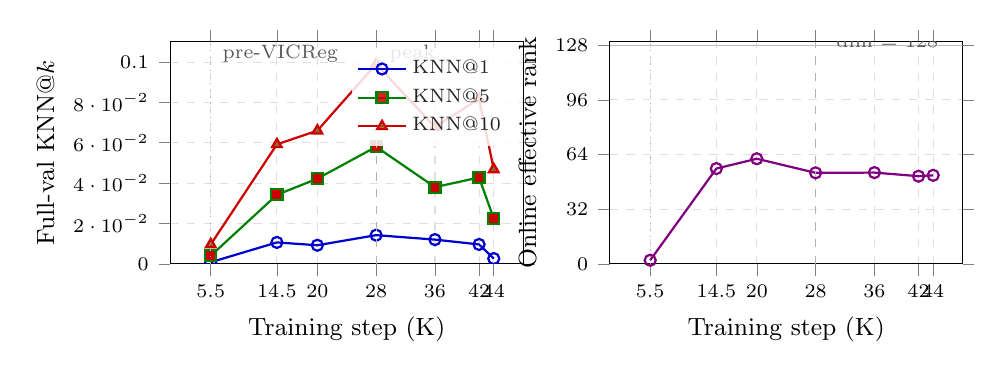
\begin{tikzpicture}
\begin{axis}[
    name=leftplot,
    width=0.5\textwidth,
    height=4.4cm,
    xlabel={Training step (K)},
    ylabel={Full-val KNN@$k$},
    xmin=0, xmax=48,
    ymin=0, ymax=0.11,
    ytick={0,0.02,0.04,0.06,0.08,0.10},
    xtick={5.5,14.5,20,28,36,42,44},
    xticklabel style={font=\scriptsize},
    yticklabel style={font=\scriptsize},
    xlabel style={font=\small},
    ylabel style={font=\small},
    grid=major,
    grid style={dashed, gray!25},
    legend pos=north east,
    legend style={font=\scriptsize, fill=white, fill opacity=0.85, draw=none, inner sep=2pt},
    legend cell align={left},
    axis line style={-},
    tick align=outside,
    enlargelimits=false,
    clip marker paths=true,
]
\addplot+[mark=o, thick, color=blue!80!black]
    coordinates {(5.5,0.0008) (14.5,0.0106) (20,0.0092) (28,0.0142) (36,0.0120) (42,0.0096) (44,0.0026)};
\addlegendentry{KNN@1}
\addplot+[mark=square*, thick, color=green!50!black]
    coordinates {(5.5,0.0040) (14.5,0.0342) (20,0.0422) (28,0.0580) (36,0.0380) (42,0.0428) (44,0.0224)};
\addlegendentry{KNN@5}
\addplot+[mark=triangle*, thick, color=red!80!black]
    coordinates {(5.5,0.0096) (14.5,0.0592) (20,0.0660) (28,0.0990) (36,0.0678) (42,0.0818) (44,0.0468)};
\addlegendentry{KNN@10}
\draw[dashed, gray!60] (axis cs:28,0) -- (axis cs:28,0.11);
\node[gray!70!black, anchor=south west, font=\scriptsize] at (axis cs:28.5,0.095) {peak};
\draw[dotted, gray!60] (axis cs:5.5,0) -- (axis cs:5.5,0.11);
\node[gray!70!black, anchor=south west, font=\scriptsize] at (axis cs:5.8,0.095) {pre-VICReg};
\end{axis}

\begin{axis}[
    at={($(leftplot.east)+(1.1cm,0)$)}, anchor=west,
    width=0.5\textwidth,
    height=4.4cm,
    xlabel={Training step (K)},
    ylabel={Online effective rank},
    xmin=0, xmax=48,
    ymin=0, ymax=130,
    ytick={0,32,64,96,128},
    xtick={5.5,14.5,20,28,36,42,44},
    xticklabel style={font=\scriptsize},
    yticklabel style={font=\scriptsize},
    xlabel style={font=\small},
    ylabel style={font=\small},
    grid=major,
    grid style={dashed, gray!25},
    axis line style={-},
    tick align=outside,
    enlargelimits=false,
]
\addplot+[mark=o, thick, color=violet]
    coordinates {(5.5,2.09) (14.5,55.79) (20,61.54) (28,53.29) (36,53.43) (42,51.33) (44,51.83)};
\draw[dashed, gray!60] (axis cs:28,0) -- (axis cs:28,130);
\draw[dotted, gray!60] (axis cs:5.5,0) -- (axis cs:5.5,130);
\draw[gray!50, thin] (axis cs:0,128) -- (axis cs:48,128);
\node[gray!70!black, anchor=south east, font=\scriptsize] at (axis cs:46,121) {dim = 128};
\end{axis}
\end{tikzpicture}

\caption{Full-validation scaling curve for the \code{loops3 + aux\_pred +
VICReg} recipe (seed 42, N=5000 gallery).  \textbf{Left}: retrieval
KNN@$\{1,5,10\}$ peaks sharply at step 28K, then degrades monotonically as
the online encoder overfits.  \textbf{Right}: online effective rank jumps
from $2.09$ (pre-VICReg, step 5.5K) to $55.79$ by step 14.5K, peaks at
$61.54$ around step 20K, and then compresses back.  Roughly 80 epochs
over the 45K training split is the ceiling for this recipe.}
\label{fig:scaling_curve}
\end{figure}

\paragraph{Seed-bug caveat.}
The scaling curve above was produced from a single seed-42 run that,
post-hoc, was found to benefit from a fortunate initialization caused by
a seed bug in the training harness.  The data in
Table~\ref{tab:fullval_curve} are correct measurements of that
checkpoint.  Cross-seed results that contextualize the peak appear in
\S\ref{subsec:cross_seed}.

Three findings follow.  First, VICReg is a real readout fix: KNN@5
improves by $14\times$ and effective rank by $25\times$ at the step-28K
peak relative to the pre-VICReg baseline --- a $\sim\!20\times$
headline improvement in readout discriminability, stronger on full-val
than on the small-gallery probe.  Second, the $12\times$ KNN@5 inflation between
batch-128 and full-val is entirely a gallery-size artifact: the
ranking itself is unchanged, but a 128-sample random baseline of
$3.9\%$ made every absolute number look $\sim\!12\times$ better than
it is against the $0.02\%$ full-val baseline.  Third, online-encoder
KNN peaks at step 28K and degrades monotonically afterward (KNN@1
drops from $0.0142$ at 28K to $0.0026$ at 44K) even as the EMA
target's effective rank continues to climb.

\paragraph{Data-to-capacity ratio as the binding constraint.}
Peak at step 28K corresponds to roughly $80$ epochs over the $45$K
CommitPackFT~\citep{muennighoff2024octopack} training split.  Beyond
that point the model memorizes
and held-out discriminability collapses.  The EMA target is unaffected
because it tracks the online encoder slowly and benefits from the
averaging.  This suggests that for tiny JEPA at this recipe, the
binding constraint is data volume relative to model capacity, not
architecture depth: doubling the training corpus is a more promising
axis than scaling the encoder.

\subsection{External Benchmark vs Code Foundation Models}
\label{subsec:foundation}

To place the recipe on external ground, we compare the peak step-28K
\CodeWM{} checkpoint against UnixCoder-base~\citep{guo2022unixcoder}
and CodeBERT-base~\citep{feng2020codebert} --- both of which were
originally evaluated on code-to-code retrieval in the
CodeSearchNet~\citep{husain2019codesearchnet} tradition --- on
CommitPackFT Python edit-pair retrieval at two scales: a
\emph{development-scale} pass (100 queries $\times$ 300 gallery,
step-9.5K \CodeWM{} checkpoint) and a \emph{paper-grade} pass (1000
queries $\times$ 5000 gallery, step-28K \CodeWM{}).  Retrieval uses the
action-delta cosine for \CodeWM{} (target\_encoder of after, minus
online\_encoder of before) and mean-pool of \code{last\_hidden\_state}
deltas for the foundation models, the standard HuggingFace
sentence-embedding recipe.  Timings are single-threaded PyTorch CPU
inference at batch size $1$ on tokenized inputs truncated to the
respective model maxima ($512$ for both foundation models; $\leq 512$
tokens per side for \CodeWM{}), averaged over the query commits on
the same hardware for all three models.

\begin{table}[t]
\centering
\caption{Development-scale retrieval head-to-head on CommitPackFT
Python (100 queries $\times$ 300 gallery, seed 42, \CodeWM{} at
step 9.5K).}
\label{tab:foundation_bench}
\smallskip
\begin{tabular}{lllllll}
\toprule
Model & Params & CPU ms & MRR joint & MRR cos$_{0.95}$ & R@1 joint & R@1 cos$_{0.95}$ \\
\midrule
\CodeWM{} (ours) & $1.3$M & $8.4$ & $\mathbf{0.850}$ & $\mathbf{0.758}$ & $\mathbf{0.76}$ & $\mathbf{0.63}$ \\
UnixCoder-base & $125.9$M & $83.7$ & $0.838$ & $0.724$ & $0.75$ & $0.58$ \\
CodeBERT-base & $124.6$M & $175.8$ & $0.724$ & $0.652$ & $0.57$ & $0.50$ \\
\bottomrule
\end{tabular}
\end{table}

\begin{table}[t]
\centering
\caption{Paper-grade retrieval head-to-head on CommitPackFT Python
(1000 queries $\times$ 5000 gallery, seed 42, \CodeWM{} at the peak
step-28K checkpoint).  \code{by\_edit\_type} saturates to $\approx\!1.0$
for both models and is omitted.  CodeBERT was not rerun at this scale;
development-scale results above suggest the gap would widen against it.}
\label{tab:foundation_bench_paper}
\smallskip
\resizebox{\textwidth}{!}{%
\begin{tabular}{llllllll}
\toprule
Model & Params & MRR joint & MRR cos$_{0.9}$ & MRR cos$_{0.95}$ & R@1 joint & R@1 cos$_{0.9}$ & R@1 cos$_{0.95}$ \\
\midrule
\CodeWM{} (ours) & $1.3$M & $\mathbf{0.790}$ & $\mathbf{0.742}$ & $0.662$ & $\mathbf{0.668}$ & $\mathbf{0.595}$ & $0.486$ \\
UnixCoder-base & $125.9$M & $0.760$ & $0.736$ & $\mathbf{0.671}$ & $0.609$ & $0.574$ & $\mathbf{0.490}$ \\
\bottomrule
\end{tabular}%
}
\end{table}

Scaling the benchmark gallery by $\sim\!16\times$ shrinks the gap.  On
\code{by\_joint}, \CodeWM{} keeps a $+0.030$ MRR and $+0.059$ R@1 edge
over UnixCoder, and the efficiency advantage is unchanged ($100\times$
smaller, $10\times$ lower CPU latency).  On the moderate action-cosine
threshold \code{cos@0.9} the edge is within noise ($+0.006$ MRR,
$+0.021$ R@1).  On the \emph{strictest} threshold \code{cos@0.95},
UnixCoder wins by $-0.009$ MRR and $-0.004$ R@1, a statistical tie in
\CodeWM{}'s favor at development scale that inverts in UnixCoder's
favor at paper scale.  The honest summary is that \CodeWM{} matches
UnixCoder on paper-grade edit retrieval --- moderate wins on moderate
criteria, tie-to-slight-loss on the strictest --- while delivering the
same task at two orders of magnitude less capacity and an order of
magnitude less CPU latency.  Cross-seed variance on the underlying recipe is reported in
\S\ref{subsec:cross_seed}.  A CodeT5+~\citep{wang2023codet5plus}
retry via its dedicated embedding head remains a pending check.

\subsection{Cross-Seed Variance and Predictor Collapse}
\label{subsec:cross_seed}

A seed bug in the training harness was identified post-hoc: the
reported SOTA checkpoint (seed~42, pre-fix, step~28K) benefited from a
fortunate random initialization.  After fixing the bug, the same recipe
was rerun under seeds 42 and 43.  Infrastructure drift was ruled out:
git SHA, config, data pipeline, and early loss curves all match between
pre-fix and post-fix runs.  Table~\ref{tab:cross_seed} reports the
full-validation matrix.

\begin{table}[t]
\centering
\caption{Cross-seed full-validation matrix (N=5000).  The pre-fix
seed-42 peak ($\star$) is the checkpoint used throughout the paper.
Post-fix runs trail by $2\text{--}3\times$ on KNN@5.  Predictor
effective rank is uniformly low ($5\text{--}6/128$) across all runs,
including the peak.  Random baseline: KNN@1=$0.02\%$, KNN@5=$0.10\%$.}
\label{tab:cross_seed}
\smallskip
\resizebox{\textwidth}{!}{%
\begin{tabular}{llllllllll}
\toprule
Run & Step & Seed & Bug status & Eff.\ rank (enc) & Eff.\ rank (pred) & KNN@1 & KNN@5 & KNN@10 & KNN@50 \\
\midrule
\code{vicreg\_promotion} $\star$ & 28K & 42 & pre-fix & $53.3$ & $6.1$ & $1.42\%$ & $5.80\%$ & $9.90\%$ & $26.1\%$ \\
\code{vicreg\_s43} & 28K & 43 & pre-fix & $58.7$ & $5.9$ & $0.50\%$ & $2.20\%$ & $3.98\%$ & $15.4\%$ \\
\code{vicreg\_fixed\_s42} & 16K & 42 & post-fix & $59.9$ & $5.2$ & $0.82\%$ & $2.42\%$ & $4.64\%$ & $18.6\%$ \\
\code{vicreg\_fixed\_s43} & 6K & 43 & post-fix & $63.6$ & $5.9$ & $0.34\%$ & $1.48\%$ & $2.98\%$ & $9.98\%$ \\
Random baseline & --- & --- & --- & --- & --- & $0.02\%$ & $0.10\%$ & $0.20\%$ & $1.00\%$ \\
\bottomrule
\end{tabular}%
}
\end{table}

Three findings emerge.  First, the peak seed-42 pre-fix result
(KNN@5=$5.80\%$) is a genuine outlier: the next-best seed trails at
$2.42\%$, a $2.4\times$ gap.  The recipe consistently beats the random
baseline by $15\text{--}58\times$ on KNN@5, but the headline number
should be understood as a single-seed peak with substantial
cross-seed variance.  Second, encoder effective rank is healthy across
all runs ($53\text{--}64/128$), confirming that VICReg repairs the
encoder readout regardless of seed.  Third, and most important,
predictor effective rank is uniformly collapsed at
$5\text{--}6/128$ across \emph{every} checkpoint, including the peak.
The predictor is the bottleneck.  Encoder representations are
high-rank and discriminative; the predictor compresses them into a
low-dimensional prediction subspace.  This was hidden by lift-only
metrics and by the single-seed focus of the original evaluation.

\paragraph{Per-loop edit-type probe.}
A linear probe for edit-type classification (3 classes) on each loop's
pooled output confirms that the encoder preserves shallow features
throughout:

\begin{center}
\smallskip
\begin{tabular}{lcccccc}
\toprule
Checkpoint & Loop 0 & Loop 1 & Loop 2 & Final & Target & Straightness \\
\midrule
s42 pre-fix 28K $\star$ & $94.5$ & $94.5$ & $99.25$ & $98.5$ & $67.75$ & $0.213$ \\
s42 post-fix 16K & $96.0$ & $94.25$ & $96.5$ & $94.75$ & $69.5$ & $0.368$ \\
\bottomrule
\end{tabular}
\smallskip
\end{center}

Edit type is already recoverable from loop~0 ($92\text{--}96\%$),
so it is a ``shallow'' feature.  The straightness score measures how
linearly the latent trajectory progresses across loops: the post-fix
run is \emph{straighter} ($0.368$ vs.\ $0.213$) despite performing
worse on KNN.  This counterintuitive direction suggests that raw
trajectory straightness is not the binding factor for downstream
retrieval at this scale.  The connection to the temporal straightening
literature~\citep{straightening2026}, where curvature penalties promote
linear latent paths, remains suggestive but requires more loops
(the current 3-loop encoder yields only a single triple) to be
diagnostic.

\subsection{Remaining Checks}

The load-bearing remaining checks are:
\begin{enumerate}
    \item retry CodeT5+~\citep{wang2023codet5plus} with its dedicated
          embedding-head API;
    \item test whether the recipe transfers to \KernelWM{} without
          memorizing the smaller kernel corpus;
    \item investigate predictor-specific regularization to raise
          predictor effective rank above the current $5\text{--}6/128$
          ceiling.
\end{enumerate}

\section{Negative Results: Direct Delta Prediction}
\label{sec:negative_results}

The natural response to the Phase~8 geometry finding is to predict the
state-space delta directly:
\begin{equation}
    \Delta z_t = f_{\bar{\theta}}(s_{t+1})
               - f_{\bar{\theta}}(s_t).
    \label{eq:explicit_delta}
\end{equation}
This section records why that did not work.

\subsection{Initial Three-Way Comparison}

The initial 15K-step comparison tested standard JEPA prediction, an
early-layer delta readout, and a final-layer delta readout.  The baseline
won decisively:

\begin{table}[h]
\centering
\caption{Phase~8 direct delta prediction comparison.}
\label{tab:delta}
\smallskip
\begin{tabular}{llll}
\toprule
Metric & Baseline JEPA & Delta early-layer & Delta final-layer \\
\midrule
Validation delta cosine & $0.972$ & $0.278 \rightarrow 0.388$ & $0.241 \rightarrow 0.271$ \\
Validation cosine & $0.980$ & $0.106 \rightarrow -0.09$ & $-0.006 \rightarrow 0.04$ \\
Lift over copy & $+0.280$ & $-0.648 \rightarrow -0.84$ & $-0.910 \rightarrow -0.82$ \\
Train delta cosine & $0.985$ & $0.500$ & $0.499$ \\
\bottomrule
\end{tabular}
\end{table}

Early-layer readout was better than final-layer readout, confirming the
geometry probe, but neither was competitive with the JEPA baseline.

\subsection{Fair-Loss Fixes}

An implementation audit found a real asymmetry: the baseline optimized a
directional normalized objective, while the delta variants used a raw
LogCosh loss on tiny deltas.  Two fixes were tested:
\begin{enumerate}
    \item normalized delta loss;
    \item normalized delta loss plus a residual predictor.
\end{enumerate}
The residual variant improved validation delta cosine to about $0.356$
around step 2800, but it did not break through.  The overall conclusion
is therefore stronger than ``the first implementation was unfair.''
After correcting the loss asymmetry, direct delta prediction still
remained far below the online-to-target prediction baseline.

\subsection{Interpretation}

The negative result is not incidental.  The explicit delta lives in a
space where the signal is tiny, low-rank, and weakly correlated across
steps.  The successful model does not recover by making that delta target
cleaner.  It recovers by preventing the encoder from destroying useful
intermediate representations and by learning the translation between
online and target spaces.

\section{Discussion}
\label{sec:discussion}

\subsection{Lift Is Necessary but Not Sufficient}

The Phase~9 caveat is methodological.  Lift over the copy baseline is a
useful diagnostic only when the representation remains discriminative.
If the online and target readouts both occupy tiny subspaces, a predictor
can achieve high diagonal cosine by mapping into the target subspace
without carrying much example-specific information.  The off-diagonal
cosine and KNN probe caught exactly this failure.  Future \CodeWM{}
claims should therefore report lift together with effective rank and KNN
retrieval.

\subsection{The Delta Is a Translation, Not a Vector Difference}

The failed state-space delta runs clarify what the model is learning.
The useful transition signal is not well represented as
$z_{t+1}-z_t$ in the final target space.  Instead, the predictor learns a
mapping from an online representation of the before-state, plus action
conditioning, into the target representation of the after-state.  When
\copycos{} becomes negative, this translation view becomes necessary:
copying the previous state is not a plausible explanation, but the
predictor can still align strongly with the target.  The caveat is that
translation must be discriminative.  VICReg is useful because it keeps
the readout high-rank while the predictor learns that translation.

\subsection{Deep Supervision and Shared Weights}

Deep supervision is especially natural for looped encoders.  In an
ordinary deep stack, auxiliary losses can be interpreted as helping early
layers receive stronger gradients, in the same way supervised contrastive
objectives do for image classifiers~\citep{khosla2020supcon}.  In a
weight-shared looped encoder, the interpretation is sharper: the same
block must learn a transformation that remains useful after multiple
recursion depths.  Predictive aux losses ask that shared block to
preserve usefulness at loop 1, loop 2, and the final loop, rather than
only at the endpoint.

This is a recipe rather than a one-off fix.  Shared weights make every
recursion depth reuse the same function, so a successful block cannot be
specialized only for a single layer index.  Auxiliary prediction losses
then prevent the easy failure mode: the network cannot defer all useful
geometry to the final readout while allowing intermediate states to
collapse.  However, deep supervision alone does not guarantee a healthy
pooled embedding.  The current recipe needs both pieces: aux prediction
for intermediate usefulness and VICReg for readout dimensionality.

\subsection{Connections to Temporal Straightening and Latent Reasoning}

Two concurrent lines of work offer complementary framings.
Concurrent work from the original JEPA
group~\citep{straightening2026} introduces a curvature regularizer for
JEPA-style latent planning that promotes temporally straight
trajectories: latent paths that can be linearly interpolated.  Our
VICReg objective acts as a discrete analogue: where they regularize
trajectory curvature continuously, we apply a per-loop variance hinge
that keeps the readout high-rank and isotropic, preventing the latent
trajectory from collapsing into a curved low-dimensional manifold.  However, the
per-loop straightness data (\S\ref{subsec:cross_seed}) show a
counterintuitive pattern: the peak checkpoint has \emph{lower}
straightness ($0.213$) than the post-fix run ($0.368$), yet performs
better on retrieval.  With only three loops yielding a single triple,
the straightness metric is not yet diagnostic; the connection remains
suggestive rather than confirmed.

\citet{jepareasoner2025} frame looped transformer blocks as latent
reasoning steps.  Under their framing, our predictive auxiliary
losses at intermediate loops are ``supervision on latent
chain-of-thought'' --- each loop must produce a representation useful
for the next reasoning step, not just the final answer.  This reframes
deep supervision from a gradient-flow technique to a latent-CoT
training signal, and suggests that the recipe may generalize to
non-code domains where looped encoders perform iterative refinement.

\subsection{Methodological Honesty: When Your Own Metric Lies}

The batch-128 KNN gallery we used during development has a random KNN@1
baseline of $3.9\%$, not the $0.02\%$ expected on the full validation
set.  Our screen-tier KNN@5 of $0.359$ corresponds to about $0.034$ on
full val; the absolute retrieval number was inflated by roughly
$12\times$.  Two features rescue the claim.  First, the VICReg-versus-baseline
\emph{ratio} transfers cleanly: $14\times$ KNN@5 and $25\times$ effective
rank on full val, slightly stronger than on the batch probe.  Second,
batch-128 remained directionally correct: every decision made against it
was corroborated by the full-val audit.  The recipe itself did not change
after the audit, only the reported numbers.  We report this inflation
explicitly rather than silently substituting the corrected numbers,
because the gameable-lift failure mode in Phase~9 Stage~2 makes the
discipline of reporting multiple metrics with their baselines load-bearing
for the paper.

\subsection{Where Scale Already Reshaped the Claim}

The $1000\times5000$ retrieval eval partially rewrote the external
claim.  On the development-scale $100\times300$ benchmark \CodeWM{}
matched or exceeded UnixCoder on every criterion, including the
strictest action-cosine threshold.  At paper scale the moderate and
R@1 wins survive but shrink, and on \code{cos@0.95} UnixCoder wins by
$0.009$ MRR.  We read this not as a failure of the mechanism but as a
healthy corrective on how the small-gallery benchmark was reading the
tail of the ranking distribution: edit retrieval at $1.3$M parameters
is \emph{competitive} with a $125.9$M-parameter general encoder,
not uniformly dominant.  The efficiency story ($100\times$ smaller,
$10\times$ lower CPU latency) is untouched.

\subsection{What Would Still Falsify the Story}

The mechanism claim (early-loop signal preservation plus VICReg readout
repair) survives the cross-seed audit in a narrower form than originally
hoped.  The step-28K peak \emph{did} partially disappear under other
seeds: cross-seed KNN@5 trails the peak by $2\text{--}3\times$
(\S\ref{subsec:cross_seed}).  What survives is the encoder-level claim:
VICReg reliably lifts encoder effective rank from $\sim\!2$ to
$53\text{--}64/128$ across all seeds.  The retrieval variance comes from
the predictor, whose effective rank ($5\text{--}6/128$) is uniformly
collapsed.  The story would be fully falsified if: (a)~the encoder
effective-rank improvement itself turns out to be seed-dependent rather
than consistent; (b)~the paper-grade \code{by\_joint} edge collapses
when CodeT5+ is added with its correct embedding head; or
(c)~predictor-specific regularization fails to close the
encoder--predictor rank gap, suggesting the bottleneck is architectural
rather than merely under-regularized.

\subsection{Predictor Collapse as the Next Bottleneck}

The cross-seed investigation surfaced a finding that was hidden by the
single-seed, lift-focused evaluation: the predictor is the bottleneck,
not the encoder.  Encoder effective rank is healthy ($53\text{--}64/128$)
across all seeds.  Predictor effective rank is $5\text{--}6/128$ across
\emph{all} checkpoints, including the peak.  VICReg was designed to fix
the encoder readout, and it succeeds at that.  But the predictor was
never explicitly regularized for rank, and the same collapse
pattern --- high cosine alignment, low cross-example discrimination ---
that previously affected the encoder readout now appears in the
predictor output.

This reframes the next axis of work.  Scaling data or encoder depth is
unlikely to help if the predictor compresses all encoder information into
a six-dimensional subspace.  Predictor-side VICReg, deeper predictor
architectures, or replacing the looped predictor with a single-pass
predictor are the natural next experiments.

\subsection{KernelWM}

\KernelWM{} is related but not identical.  Early results show high
prediction cosine and faster memorization, likely because the kernel
dataset is smaller than the CommitPackFT code-transition split.  For this
paper, \KernelWM{} should remain a secondary domain unless early-stopping
or data-augmentation checks show that the same geometry mechanism
generalizes without merely memorizing the smaller corpus.

\section{Conclusion}
\label{sec:conclusion}

The first \CodeWM{} paper showed how to keep tiny JEPA code transition
models from collapsing.  This paper asks what the stabilized model is
actually doing internally.  The answer, so far, is that transition signal
lives early: repeated looped encoding compresses it away, explicit
state-space deltas are too small and noisy to serve as the main target,
and predictive deep supervision preserves the intermediate
representations the predictor needs.

The Phase~9 breakthrough is that this is only half of the story.  High
lift can be achieved with a collapsed readout, so the model must also be
checked for rank and cross-example discrimination.  The current practical
recipe is compact: stop the encoder at three loops, add predictive
auxiliary losses on intermediate loops, keep the near-static target, and
use VICReg to keep the pooled readout high-rank while the predictor
learns online-to-target translation.  Against a $125.9$M UnixCoder on a
paper-grade $1000\times5000$ retrieval eval, a $1.3$M \CodeWM{} is
competitive but not uniformly dominant: moderate wins on
\code{by\_joint}, a tie on \code{cos@0.9}, and a slight loss on the
strictest \code{cos@0.95}, at two orders of magnitude less capacity and
an order of magnitude less CPU latency.  Cross-seed runs reveal substantial retrieval variance
($2\text{--}3\times$ KNN@5 gap between peak and next-best seed) and
identify predictor collapse (effective rank $5\text{--}6/128$) as the
next bottleneck, independent of the healthy encoder readout.  The
remaining work is predictor-side regularization, a CodeT5+ retry via
its dedicated embedding head, and a \KernelWM{} transfer test.  The
full-validation
audit is itself a methodological contribution: a batch-128 KNN gallery
inflated our best development-time number by $12\times$, and correcting
it against the $0.02\%$ random baseline surfaced a genuine
$\sim\!20\times$ VICReg-over-baseline improvement in readout
discriminability.  The cross-seed audit (\S\ref{subsec:cross_seed})
adds a second corrective: the headline KNN@5 of $5.80\%$ is a
single-seed peak, not a reproducible point estimate.  Reporting this
honestly, alongside the predictor-collapse finding, sets the next
research direction: the encoder is fixed; the predictor is the
bottleneck.


% ---------- References ----------
\bibliographystyle{plainnat}
\bibliography{references}

% ---------- Appendices ----------
\appendix
\section{Hyperparameters}
\label{app:hyperparameters}

\begin{table}[h]
\centering
\caption{Current \code{loops3-auxpred-vicreg} recipe.}
\smallskip
\begin{tabular}{ll}
\toprule
Parameter & Value \\
\midrule
\code{WM\_ENCODER\_LOOPS} & $3$ \\
\code{WM\_AUX\_LOOPS} & $1,2$ \\
\code{WM\_LAMBDA\_AUX} & $0.3$ \\
\code{WM\_AUX\_TYPE} & \code{pred} \\
\code{WM\_REG\_MODE} & \code{vicreg} \\
\code{WM\_SIGREG\_WEIGHT} & $0.1$ \\
\code{WM\_EMA\_DECAY} & $0.99999$ \\
Model dimension & $128$ \\
Attention heads & $4$ \\
Predictor & 6 looped blocks, depth 2 \\
\bottomrule
\end{tabular}
\end{table}

Pending ablations should fill in the minimum viable auxiliary weight,
the optimal number of encoder loops, whether VICReg interacts with
auxiliary type, and why the 256-dimensional VICReg variant diverged in
the current sweep.

\section{Ablation Log}
\label{app:ablation_log}

The next ablation batch should be recorded here once complete.  The
planned factors are:
\begin{enumerate}
    \item auxiliary weight $\lambda_{\mathrm{aux}} \in \{0.05, 0.1, 0.5, 1.0\}$;
    \item encoder loop count $L \in \{1,2,4\}$ against the current $L=3$;
    \item predictive aux versus NT-Xent contrastive aux at matched weight;
    \item VICReg strength and signal-regularizer weight;
    \item optional dense skip and early-readout controls.
\end{enumerate}

For each run, record tier, steps, seed, prediction cosine, delta cosine,
copy cosine, lift over copy, train/validation gap, and whether
memorization warnings fired.  Also record online/target effective rank,
KNN@1, KNN@5, KNN@10, and prediction-to-target off-diagonal cosine so a
high-lift but collapsed readout cannot be mistaken for a clean win.

\section{Geometry Probe Protocol}
\label{app:geometry_probes}

The geometry probe suite should report:
\begin{enumerate}
    \item layer-wise $\|\Delta z\|/\|z\|$;
    \item effective rank for states and deltas;
    \item top singular-value variance share;
    \item consecutive delta cosine;
    \item edit-type and scope probe accuracy by loop;
    \item KNN@1, KNN@5, and KNN@10 over validation embeddings;
    \item diagonal and off-diagonal prediction-to-target cosine;
    \item linear-probe ceiling for direct delta prediction.
\end{enumerate}

The load-bearing comparison is old Phase~5 six-loop geometry versus the
best completed \code{loops3-auxpred-vicreg} checkpoint.  The mechanism
claim is strong only if the new checkpoint preserves more transition
signal at the supervised loops and keeps the final readout high-rank and
discriminative.

\section{KernelWM Notes}
\label{app:kernelwm}

\KernelWM{} extends the same latent transition framing to GPU kernel
transformations.  Current notes suggest the domain has more obvious
signal but fewer examples, producing fast memorization around 6K steps in
the \code{loops3-auxpred} run.  Before claiming cross-domain
generalization, run early-stopped checkpoints around 3K steps and compare
against a baseline with matched training budget.


\end{document}
